\begin{frame}{Signal Protocol}
    \framesubtitle{Il protocollo: X3DH}
    X3DH è stato sviluppato da OWS per supportare lo scambio asincrono delle chiavi. \cite{X3DH}\pause\newline
    Definizioni:
    \begin{itemize}
        \item Identity key: chiave pubblica\pause
        \item Ephemereal key: chiave utilizzabile una sola volta \pause
        \item Pre-keys: chiavi condivise col server prima dell'attivazione del protocollo\pause
        \item One-time pre-keys: insiemi di pre-keys condivisi col server prima dell'attivazione del protocollo. Il server condivide una chiave ogni volta che un utente vuole iniziare una conversazione e ne richiede un nuovo insieme quando stanno per finire\pause
        \item Signed pre-key: pre-key firmata con l'esponente dell'Identity key
    \end{itemize}

    \note{
        STANDARD DIFFIE-HELLMAN: Alice e Bob generano ognuno una chiave pubblica \textit{pk} basata su un generatore comune \textit{g} modulo \textit{m} e le proprie chiavi private (\textit{secret keys}) \textit{sk}. \\Dopodiché scambiano le chiavi pubbliche attraverso un canale (potenzialmente non sicuro) e da esse possono derivare una chiave segreta condivisa \textit{ssk}.
        \cite{diffiehellman}, \cite{diffiehellman2}
    }
\end{frame}

\begin{frame}{Signal Protocol}
    \framesubtitle{Il protocollo: X3DH}

    \begin{figure}
        \centering
        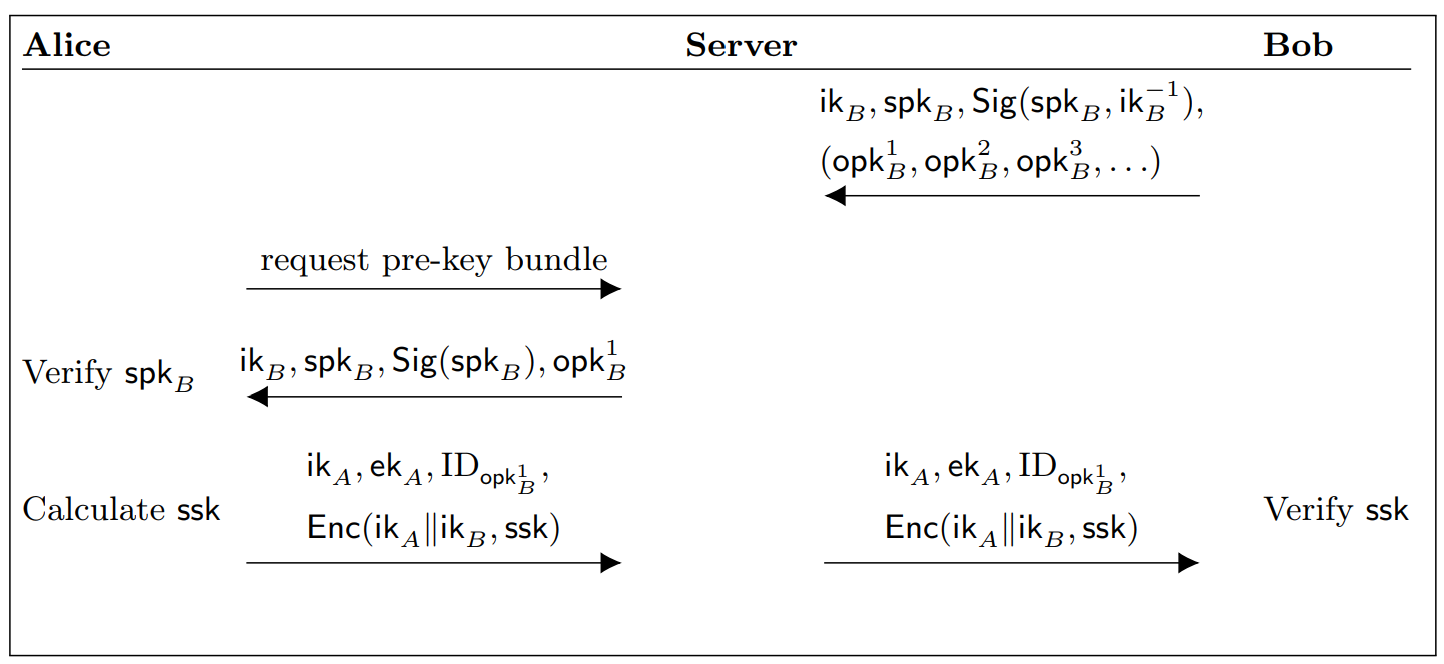
\includegraphics[width=.8\textwidth]{X3DH.png}
        \caption{Funzionamento di X3DH semplificato}
    \end{figure}

    \cite{VanDam}
\end{frame}
